\documentclass{report}
\usepackage[utf8]{inputenc}
\usepackage[portuguese]{babel}
\setcounter{secnumdepth}{5}
\usepackage{verbatim}
\usepackage{indentfirst}
\usepackage{natbib}
\usepackage{graphicx}
\usepackage{cite}
\usepackage{hyperref}


\title{Trabalho 2: Report 2007: Vamos escrever Relatórios}
\author{a61007 César Perdigão \\ a61009 Luís Caseiro \\ a61078 Pedro Maia}
\date{Junho 2013}


\begin{document}

\maketitle
\tableofcontents
\chapter{Introdução}
O objetivo deste trabalho prático nº2 é fazer com que o grupo aumenta a sua experiencia a trabalhar com gramáticas independentes de contexto através de ferramentas geradoras de compiladores como o par \textbf{lex/yacc}.

Uma  gramática independente de contexto é definida por um quatro elementos, um conjunto finito, não vazio, de simbolos não terminais, um conjunto finito não vazio de simbolos terminais, símbolo inicial da gramática e um conjunto de regras. Esta é independente de contexto pois as regras que definem um não terminal \textbf{X} não estão restritas a um contexto.

\chapter{Desenvolvimento}

\section{Escolha do enunciado}
O enunciado que o grupo escolheu foi o enunciado nº 3, \textit{Report 2007: vamos escrever relatórios}. O objetivo deste enunciado é desenvolver um compilador que aceita relatórios escritos numa determinada linguagem e gerará a respectiva versão HTML.

Esta escolha deve-se à escolha no trabalho prático nº1  do enunciado \textit{Pre-processador de Latex e HTML}, sendo estes dois muito parecidos, o que permite ao grupo aproveitar o trabalho feito anteriormente podendo também melhorar o seu desempenho neste novo trabalho.

\section{Constituintes da Gramática}

\subsection{Simbolos Não-Terminais}
Para os simbolos não terminais o grupo usou a sintaxe que foi dada pelo docente tendo  mantendo sempre a forma de escrita simples, alguns simbolos não terminais que usamos foram:

\begin{verbatim}
Figure Grafic Caption table 
TRowList TRow TDataList 
TData ParaContent entre outros.
\end{verbatim}
Estes simbolos sofreram derivações através de regras.
\subsection{Simbolos Terminais}
Como simbolos terminais tentamos faze-los de uma forma simples, algumas delas são:

\begin{verbatim}
BREPORT EREPORT BFM EFM BTITLE
ETITLE BSUBTITLE ESUBTITLE BAUTHOR
EAUTHOR BNAME ENAME 
EITERM BBOLD EBOLD BITALIC EITALIC 
BUNDERLINE EUNDERLINE BFIG EFIG 
BGRAPH EGRAPH BCAPTION ECAPTION
BTABLE ETABLE BTROW ETROW BTDATAETDATA TEXTO 
BDATE EDATE BINST EINST BKEYW EKEYW 
\end{verbatim}
\subsection{Regras}
O grupo usou regras simples e parecidas com a sintaxe dada de forma a facilitar o resultado. Alguns exemplos de regras são:
\begin{verbatim}
Table -> Caption TRowList

TRowList -> TRowList TRow
          | TRow
          
TRow -> BTROW TDataList ETROW

TDataList -> TDataList TData
          | TData

TData -> BTDATA ParaContent ETDATA

ParaContent -> ParaContent TEXTO
            | ParaContent FreeElem
            | &

FreeElem -> Ref
         |Bold
	     |Italic
    	 |Underline
	     |InlineCode
	     |Acronym;

\end{verbatim}

\section{Sintaxe Usada}
Para facilitar o desenvolvimento do trabalho o grupo optou por usar uma sintaxe parecida com a sintaxe \textbf{XML}.
\subsection{Cabeçalho ou FrontMatter}
Para o cabeçalho especificamos os seguintes comandos:
\begin{itemize}
\item Iniciar FrontMatter
\begin{verbatim} <fm>ConteudoFM</fm> \end{verbatim}
O conteudo fm tem \textbf{tags} título, subtitulo, autor, data, Resumo e Agradecimentos.
\item Título
\begin{verbatim} <title>titulodocumento</title> \end{verbatim} 
\item Subtítulo
\begin{verbatim} <subtitle>Subtitulodocumento</subtitle> \end{verbatim} 
\item Autor é constituido por:
\begin{itemize}
\item Nome
\begin{verbatim} <name>NomeAutor</name> \end{verbatim} 
\item Identificação
\begin{verbatim} <nident>NIAutor</nident> \end{verbatim} 
\item Email
\begin{verbatim} <email>emailAutor</email> \end{verbatim} 
\item Url
\begin{verbatim} <url>URLAutor</url> \end{verbatim} 
\item Afiliação
\begin{verbatim} <affiliation>AfiliAutor</affiliation> \end{verbatim}
\end{itemize}
\item Data
\begin{verbatim} <date>Data</date> \end{verbatim} 
\item Instituição
\begin{verbatim} <inst>Instituição</inst> \end{verbatim} 
\item Palavras Chave
\begin{verbatim} <keyw>PalavrasChave</keyw> \end{verbatim} 
\item Resumo
\begin{verbatim} <abs>Resumo</abs> \end{verbatim} 
Em que Resumo é \textit{paralist}, ou seja, uma lista de paragrafos.
\item Agradecimentos
\begin{verbatim} <akn>Agradecimentos</akn> \end{verbatim} 
Em que Agradecimentos é \textit{paralist}, ou seja, uma lista de paragrafos.
\item Índice de Conteudos
\begin{verbatim} <toc/> \end{verbatim} 
Em que esta marca sinaliza que deve ser inserida a tabela de conteudos.
\item Índice de figuras
\begin{verbatim} <lof/> \end{verbatim} 
Em que esta marca sinaliza que deve ser inserida a lista de figuras.
\item Índice de tabelas
\begin{verbatim} <lot/> \end{verbatim} 
Em que esta marca sinaliza que deve ser inserida a lista de tabelas.
\end{itemize}
\subsection{Body}
\begin{itemize}
\item Iniciar Body
\begin{verbatim} <body>ConteudoBody</body> \end{verbatim}
O conteudo Body é constituido por uma lista de Capitulos.
\item Capitulos
\begin{verbatim} <chap><title>NomeCapitulo</title>ConteudoCapitulo</chap> \end{verbatim} 
Em que o ConteudoCapitulo pode ser composto por secções, paragrafos, figuras e tabelas.
\item Secção
\begin{verbatim} <sec><title>NomeSecção</title>ConteudoSeccao</sec> \end{verbatim} 
Em que o ConteudoSeccao pode ser composto por paragrafos, figuras e tabelas.
\item Paragrafos
\begin{verbatim} <para>ConteudoParagrafo</para> \end{verbatim} 
Em que o ConteudoParagrafo pode ser composto por referencias e texto.

\item Acronimo
\begin{verbatim} <acron>Acronimo</acron> \end{verbatim} 

\item Lista de items
\begin{verbatim} <list>LItems</list> \end{verbatim}
LItems são compostos por items 
\begin{verbatim} <item>Item</item> \end{verbatim}

\item Imagens
\begin{verbatim}<fig><graph>PathFig</graph><caption>Legenda</caption></fig>\end{verbatim}

\item Tabelas

\begin{verbatim}
<table>
<caption>Legenda</caption>
<trow><tdada>ConteudoCelula</tdata></trow>
</table>
\end{verbatim}
\end{itemize}

\subsection{Texto Formatado}
\begin{itemize}
\item Negrito 
\begin{verbatim} <bold>PalavrasaNegrito</bold>  \end{verbatim}
\item Italico
\begin{verbatim} <italic>PalavrasaItalico</italic> \end{verbatim}
\item Sublinhado
\begin{verbatim} <underline>PalavrasSublinhadas</underline> \end{verbatim}


\begin{verbatim} <ref>Referencia</ref> \end{verbatim}

\end{itemize}

\subsection{Texto Não Formatado}
\begin{itemize}
\item Verbatim de linha
\begin{verbatim} <codel>Linha</codel> \end{verbatim}
\item Verbatim
\begin{verbatim} <code>Texto</code> \end{verbatim}
\end{itemize}
\chapter{Testes e Resultados}

\section{Resultados do ficheiro de teste}
Os resultados do ficheiro teste que se enconta em anexo foram:

\begin{figure}[h!]
\centering
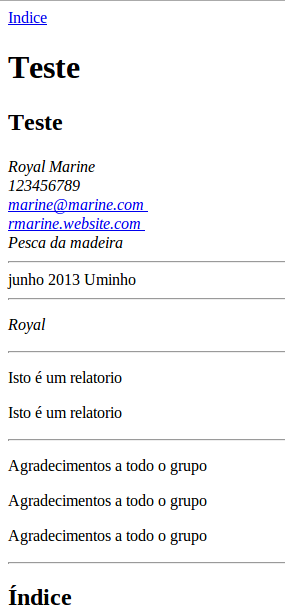
\includegraphics[scale=0.3]{HTML1.png}
\caption{Resultados do Teste parte 1}
\label{threadsVsSync}
\end{figure}

\begin{figure}[h!]
\centering
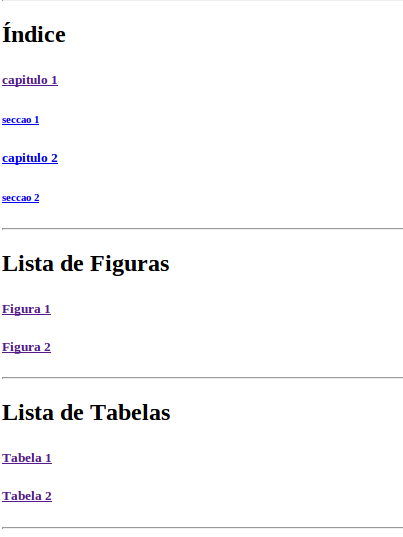
\includegraphics[scale=0.3]{HTML2.png}
\caption{Resultados do Teste parte 2}
\label{threadsVsSync}
\end{figure}

\begin{figure}[h!]
\centering
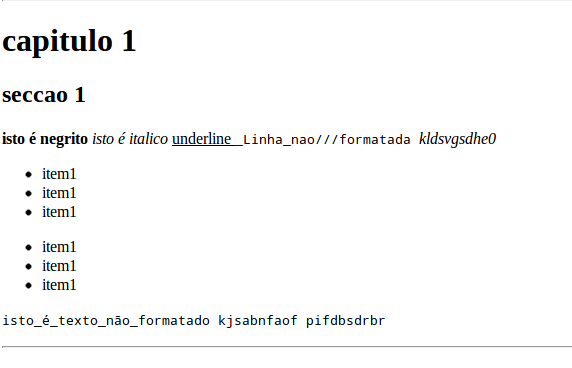
\includegraphics[scale=0.3]{HTML3.JPG}
\caption{Resultados do Teste parte 3}
\label{threadsVsSync}
\end{figure}

\begin{figure}[h!]
\centering

\includegraphics[scale=0.3]{HTML4.JPG}
\caption{Resultados do Teste parte 4}
\label{threadsVsSync}
\end{figure}

\begin{figure}[h!]
\centering
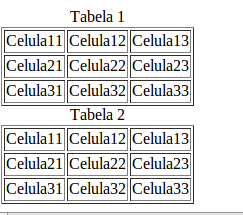
\includegraphics[scale=0.3]{HTML5.JPG}
\caption{Resultados do Teste parte 5}
\label{threadsVsSync}
\end{figure}

\chapter{Conclusão}
Após a conclusão do projeto e de analisar os resultados do teste efetuado o grupo concluiu que a relização do trabalho fez com que as suas habilidades com a utilização de gramáticas independentes de contexto evoluisse e também houve uma melhoria na performace com o par de ferramentas \textbf{lex/yacc}.

O objetivo principal foi cumprido permitindo assim ao grupo utilizar o compilador implementado para a realização de relatorios em HTML, o que pode vir a ser útil no futuro.

O maior contratempo na realização do projeto foi a existencia de múltiplos trabalhos de outras unidades curriculares que fez com que o grupo atrasasse um pouco e não conseguisse fazer alguns extras que eram sugeridos no enunciado.

\chapter{Anexos}
\section{Ficheiro de teste}
\begin{verbatim}
<report>
<fm>
    <title>
    	Teste
	</title>
	<subtitle>
		Teste
	</subtitle>
	<author>
		<name>
			Royal Marine
		</name>
		<nident>
			123456789
		</nident>
		<email>
			marine@marine.com
		</email>
		<url>
			rmarine.website.com
		</url>
		<affiliation>
			Pesca da madeira
		</affiliation>
	</author>
	<date>
		junho 2013
	</date>
	<inst>
		Uminho
	</inst>
	<keyw>
		Royal
	</keyw>
	<abs>
		<para>
			Isto é um relatorio
		</para>
		<para>
			Isto é um relatorio
		</para>
	</abs>
	<akn>
		<para>
			Agradecimentos a todo o grupo
		</para>
		<para>
			Agradecimentos a todo o grupo
		</para>
		<para>
			Agradecimentos a todo o grupo
		</para>
	</akn>
	<toc/>
	<lof/>
	<lot/>
</fm>
<body>
	<chap>
		<title>
			capitulo 1
		</title>
		<sec>
			<title>
			seccao 1
			</title>
			<para>
				<bold> isto é negrito </bold>
				<italic> isto é italico </italic>
				<underline> underline </underline>
				<codel> _Linha_nao///formatada </codel>
			</para>
			<acron>
				
			</acron>
			<list>
				<item>
					item1
				</item>
				<item>
					item1
				</item>
				<item>
					item1
				</item>
			</list>
			<list>
				<item>
					item1
				</item>
				<item>
					item1
				</item>
				<item>
					item1
				</item>
			</list>
			<code>
				isto_é_texto_não_formatado
			</code>
		</sec>		
	</chap>
	<chap>
		<title>
			capitulo 2
		</title>
		<sec>
			<title>
			seccao 2
			</title>
			<fig>
				<graph>
					/home/cesar/Imagens/piano.jpg
				</graph>
				<caption>
					Figura 1
				</caption>
			</fig>
			<fig>
				<graph>
					/home/cesar/Imagens/piano.jpg
				</graph>
				<caption>
					Figura 2
				</caption>
			</fig>
			<table>
				<caption>
					Tabela 1
				</caption>
				<trow>
					<tdata>
						Celula11
					</tdata>
					<tdata>
						Celula12
					</tdata>
					<tdata>
						Celula13
					</tdata>
				</trow>
				<trow>
					<tdata>
						Celula21
					</tdata>
					<tdata>
						Celula22
					</tdata>
					<tdata>
						Celula23
					</tdata>
				</trow>
				<trow>
					<tdata>
						Celula31
					</tdata>
					<tdata>
						Celula32
					</tdata>
					<tdata>
						Celula33
					</tdata>
				</trow>			
			</table>
			<table>
				<caption>
					Tabela 2
				</caption>
				<trow>
					<tdata>
						Celula11
					</tdata>
					<tdata>
						Celula12
					</tdata>
					<tdata>
						Celula13
					</tdata>
				</trow>
				<trow>
					<tdata>
						Celula21
					</tdata>
					<tdata>
						Celula22
					</tdata>
					<tdata>
						Celula23
					</tdata>
				</trow>
				<trow>
					<tdata>
						Celula31
					</tdata>
					<tdata>
						Celula32
					</tdata>
					<tdata>
						Celula33
					</tdata>
				</trow>			
			</table>
		</sec>
	</chap>		
</body>
</report>
\end{verbatim}

\bibliographystyle{plain}
\bibliography{references}
Enunciado:

\url{http://elearning.uminho.pt/bbcswebdav/pid-395150-dt-content-rid-507068_1/courses/1213.8206N5_2/pl1213-tp2.pdf}

\end{document}
